\section{Funcionamiento}
\label{sec:funcionamiento}

\begin{table}[!b]
\renewcommand\tabularxcolumn[1]{m{#1}}
\caption{Código de luces del \textit{Chana Monitoring System}}
\label{tab:luces}
\begin{tabularx}{\textwidth}{ccX}
\toprule
\headingc{Color} & \headingc{Estado} & \headingc{Descripción} \\
\topruleb
  \circlefilled{red}    & \textsc{apagado}      & No se ha detectado error.\newline
                                                  Comprobar \circlefilled{yellow} y \circlefilled{green} para más datos.\\*\midrule
  \circlefilled{red}    & \textsc{fijo}         & El \MIE ha perdido conexión con el \MEE durante demasiado tiempo.\\*\midrule
  \circlefilled{red}    & \textsc{intermitente} & El \MEE ha detectado que el depósito está lleno.\\*\midrule
  \circlefilled{yellow} & \textsc{apagado}      & El \MIE ha arrancado correctamente.\newline
                                                  Comprobar \circlefilled{red} y \circlefilled{green} para más datos.\\*\midrule
  \circlefilled{yellow} & \textsc{fijo}         & El \MIE está conectado a una red wifi o está en modo gestión.\\*\midrule
  \circlefilled{yellow} & \textsc{intermitente} & El \MIE acaba de encenderse, y está esperando a recibir información del \MEE\\*\midrule
  \circlefilled{green}  & \textsc{apagado}      & No hay/ha habido conexión entre el \MIE y el \MEE.\newline
                                                  Comprobar \circlefilled{red} y \circlefilled{yellow} para más datos.\\*\midrule
  \circlefilled{green}  & \textsc{fijo}         & El \CMS funciona normalmente.\\*\midrule
  \circlefilled{green}  & \textsc{intermitente} & El \CMS funciona normalmente, pero el \MEE tiene la batería baja.\\*\bottomrule
\end{tabularx}
\end{table}

Con el objetivo de maximizar el tiempo de vida de las batería del \MEE, el \MIE es quien proporciona toda la información al usuario del \CMS a través de alarmas sonoras, las luces de notificación \circled{I2}, \circled{I3} e \circled{I4} y la pantalla LCD \circled{I1}. Las luces de notificación y las alarmas sonoras permiten comprobar el estado del \CMS de un vistazo rápido, sin necesidad de comprobar los mensajes que se muestran en la pantalla LCD \circled{I1}. La tabla~\ref{tab:luces} resume los principales estados que representan las diferentes luces de notificación.



En las siguientes subsecciones, se describe en detalle las diferentes informaciones que puede mostrar el \CMS.

\subsection{Arranque}

Cuando el \MIE se conecta a la alimentación USB, éste se enciende de forma automática, e intenta conectarse a la red wifi que haya sido configurada a través de la interfaz de gestión (ver sección~\ref{sec:gestion-avanzada}). Esto se notifica mediante la luz de notificación de configuración \circled{I3} encendida de forma fija (\circlefilled{yellow}), y mostrando el mensaje \emph{Conectando a red WiFi\ldots} en la pantalla LCD \circled{I1} tal y como muestra la figura \ref{fig:screen-conn-process}.

\begin{figure}[!b]
  \centering
  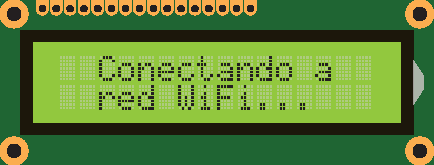
\includegraphics[width=0.6\columnwidth]{images/screen-conn-process}
  \caption{Pantalla del módulo interior -- Conectando a red wifi}
  \label{fig:screen-conn-process}
\end{figure}

\begin{figure}[!b]
  \centering
  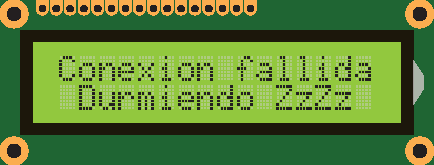
\includegraphics[width=0.6\columnwidth]{images/screen-conn-failed}
  \caption{Pantalla del módulo interior -- fallo de conexión}
  \label{fig:screen-conn-failed}
\end{figure}


En caso de que la conexión falle, el sistema apagará todas las luces de notificación y mostrará el mensaje \emph{Conexión fallida Durmiendo ZzZz} tal y como muestra la figura~\ref{fig:screen-conn-failed}. El \MI se quedará en ese estado de hibernación hasta que el usuario lo reinicie y compruebe por qué no ha sido posible realizar la conexión.



\subsection{El menú de información}

El menú de información se muestra cuendo el \MIE ha arrancado y se ha conectado a una ref wifi de forma satisfactoria. Consta de 5 pantallas, que pueden navegarse en la secuencia
~~~\tikz[baseline=-0.63ex,node distance=1em,remember picture]{
\node (n1) {1};
\node (n2) [right=of n1] {2};
\node (n3) [right=of n2] {3};
\node (n4) [right=of n3] {4};
\node (n5) [right=of n4] {5};
\draw[->] (n1) -> (n2);
\draw[->] (n2) -> (n3);
\draw[->] (n3) -> (n4);
\draw[->] (n4) -> (n5);
}
\tikz[remember picture,overlay]{
\draw[->,smooth]  (n5)
to[out=0, in=180]  ($(n5) + ( 0.3cm, 0.00cm)$)
to[out=0, in=0]    ($(n5) + ( 0.3cm,-0.22cm)$)
to[out=180,in=0]   ($(n1) + (-0.3cm,-0.22cm)$)
to[out=180,in=180] ($(n1) + (-0.3cm, 0.00cm)$)
to[out=0, in=180] (n1);
}~~
pulsando el botón multifunción \circled{I8}.

\textbf{Pasados 60 segundos desde la última pulsación del botón multifunción \circled{I8}, el \MI volverá automáticamente a la pantalla 1.}

\attbegin{Pantallas 1 y 2}
Nada más iniciarse, y mientras la luz de notificación de configuración \circled{I3} se enciende de forma \textbf{intermitente} (\circlefilled{yellow}), sólo se mostrarán las pantallas 3 a 5 hasta que el \ME realice la primera sincronización de datos y se encienda el led de notificación de conexión \circled{I4} (\circlefilled{green}). \textbf{En ese caso, al pasar 60 segundos sin pulsar el botón multifunción \circled{I8}, el \MI volverá automáticamente a la pantalla 3 en lugar de a la pantalla 1.}
\attend

Las pantallas de información que muestre el \MIE en su modo de operación normal son:

\begin{descriptioncompact}

\begin{figure}[!b]
  \centering
  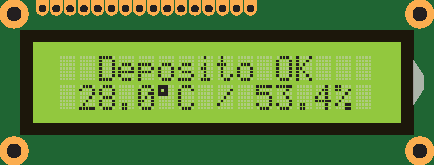
\includegraphics[width=0.6\columnwidth]{images/screen1}
  \caption{Pantalla 1 del módulo interior -- Información exterior}
  \label{fig:screen1}
\end{figure}

\item[Pantalla 1: Información exterior] --- Esta pantalla sólo se muestra cuando el \MEE ha enviado datos de estado recientemente. Como muestra la figura~\ref{fig:screen1}, la primera línea muestra el estado del depósito, mientras que la segunda línea muestra la temperatura y porcentaje de humedad exteriores.

\begin{figure}[t]
\centering
\begin{subfigure}{0.6\columnwidth}
  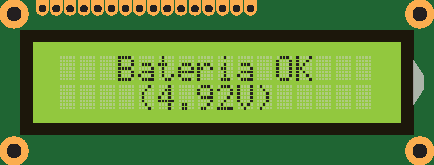
\includegraphics[width=1\columnwidth]{images/screen2a}
  \caption{}
  \label{fig:screen2a}
\end{subfigure}
\\[1em]
\begin{subfigure}{0.6\columnwidth}
  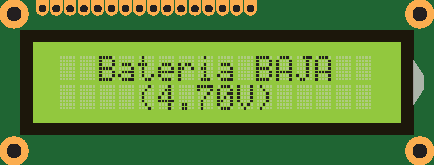
\includegraphics[width=1\columnwidth]{images/screen2b}
  \caption{}
  \label{fig:screen2b}
\end{subfigure}
\caption{Pantalla 2 del módulo interior -- información de batería}
\label{fig:screen2}
\end{figure}

\item[Pantalla 2: información de batería] --- Al igual que la pantalla 1, esta pantalla sólo se muestra cuando el \MEE ha enviado datos de estado recientemente. Como muestran la figura~\ref{fig:screen2}, la primera línea muestra el estado de la batería (según el umbral de batería baja que se haya configurado, ver sección~\ref{sec:config}), mientras que la segunda línea muestra el detalle de la tensión proporcionada por las baterías del \MEE. cuando se muestra el mensaje de \emph{Bateria BAJA}, el led de notificación de conexión \circled{I4} (\circlefilled{green}) estará encendido de forma intermitente.

\begin{figure}
  \centering
  \includegraphics[width=0.6\columnwidth]{images/screen3}
  \caption{Pantalla 3 del módulo interior -- información de red}
  \label{fig:screen3}
\end{figure}

\begin{figure}
  \centering
  \includegraphics[width=0.6\columnwidth]{images/screen4}
  \caption{Pantalla 4 del módulo interior -- IP y puerto de escucha}
  \label{fig:screen4}
\end{figure}

\begin{figure}[!b]
  \centering
  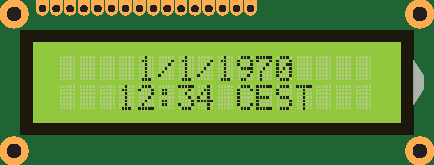
\includegraphics[width=0.6\columnwidth]{images/screen5}
  \caption{Pantalla 5 del módulo interior -- fecha y hora}
  \label{fig:screen5}
\end{figure}

\item[Pantalla 3: información de red] --- Ésta es la primera pantalla que se muestra cuan\-do el \MIE acaba de iniciarse, el \MEE todavía no ha enviado datos, y la luz de notificación de configuración \circled{I3} (\circlefilled{yellow}) todavía se enciende de forma intermitente. Como muestra la figura~\ref{fig:screen3}, en la primera línea se mostrará el nombre de la red wifi a la que se encuentre conectado el \ME (hasta un máximo de 16 caracteres), mientras que la segunda línea mostrará el nombre de host que se haya especificado en la configuración del \MI. Aquellos dispositivos que soporten el protocolo \emph{mDNS} podrán conectarse al \MI empleando el nombre de host que aquí aparece añadiendo el sufijo \emph{.local} (por ejemplo, \emph{chanams-interior.local}). 

\item[Pantalla 4: IP y puerto de escucha] --- Esta pantalla muestra más información de red. La primera línea muestra la dirección IP del \MIE ---útil en aquellos casos en los que los dispositivos que se deseen conectar no soporten el protocolo mDNS)--- mientras que la segunda línea muestra el puerto de escucha del \MI. 

\item[Pantalla 5: fecha y hora] --- Esta pantalla muestra la fecha y hora según la zona horaria que se ha establecido en las opciones de configuración (de nuevo, ver sección~\ref{sec:config}). Dadas las características del hardware del \CMS (que no dispone de reloj interno), la fecha y la hora se obtiene de internet. La primera línea muestra la fecha, mientras que la segunda línea muestra la hora y la zona horaria, por ejemplo, CEST (\textit{Central European Summer Time} u hora de verano de Europa central), CET (\textit{Central European Time} u hora de invierno de Europa central), etc.

\end{descriptioncompact}


\subsection{Avisos y alarmas sonoras}

Además de las señales luminosas, el \CMS puede lanzar avisos y alarmas sonoras para alertar de los eventos críticos que requiren de una acción inmediata del usuario. Estos avisos y alarmas son:

\begin{descriptioncompact}

\item[Aviso de batería baja] --- Cuando la tensión proporcionada por la batería del \MEE esté por debajo del umbral configurado (ver sección~\ref{sec:config}), el \MIE lo notificará regularmente emitiendo un pitido agudo en todas las horas en punto hasta que las baterías sean reemplazadas.

\item[Alarma de depósito lleno] ---  

\item[Alarma de conexión perdida] ---  


\end{descriptioncompact}

\tipbegin{Modo silencioso}
Es posible desactivar todas las alarmas sonoras de forma permanente colocando el interruptor de la alarma sonora \circled{I8} en la posición \off.
\tipend

\tipbegin{Comprobación de estado de las alarmas sonoras}
En caso de duda, es posible comprobar el estado de las alarmas sonoras pulsando el botón de reinicio \circled{I5} ---o desconectando momentáneamente la alimentación USB \circled{I6}--- del \MIE. Si las alarmas sonoras están activadas, el \CMS emitirá tres pitidos cortos al iniciarse. \textbf{Estos tres pitidos se emitiran incluso en el periodo de silencio.}
\tipend



\begin{figure}[H]
  \centering
  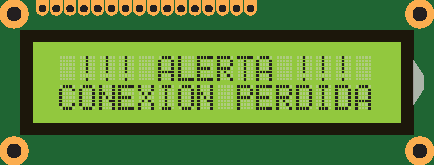
\includegraphics[width=0.6\columnwidth]{images/screen-conn-lost}
  \caption{Pantalla del módulo interior: conexión perdida}
  \label{fig:screen-conn-lost}
\end{figure}


\attbegin{En caso de conexión perdida}
En caso de que el \CMS le alerte de que se ha perdido la conexión entre en \MIE y el \MEE, proceda de la siguiente manera:

\begin{enumeratecompact}

\item \textbf{Reinicie el \MIE}. Para ello, pulse el botón de reinicio \circled{I5} ---o alterntivamente, desconecte y reconecte pasados unos segundos la alimentación USB \circled{I6}--- y espere a que el \MI informe en la pantalla LCD \circled{I1} de que se encuentra conectado a una red wifi.

\begin{itemizecompact}

\item Si tras varios intentos el \MI no se conecta a una red wifi, entre en el modo de gestión (sección~\ref{sec:gestion}, \nameref{sec:gestion}) y configure de nuevo el nombre de la red y la contraseña (sección~\ref{sec:config}, \nameref{sec:config}).

\end{itemizecompact}

\item \textbf{Reinicie el \MEE y compruebe que dispone de batería}. Para ello, coloque el interruptor de encendido \circled{E2} en la posición \off, espere unos segundos, y vuelva a conectar el \ME moviendo el interruptur de encendido \circled{E2} a la posición \on. 

\begin{itemizecompact}

\item Si la luz de notificación de actividad \circled{EI} no se enciende, reemplace las pilas del \ME, y vuelva al paso 2.

\item Si la luz de notificación de actividad \circled{EI} emite un breve destello azul, continúe. 

\end{itemizecompact}


\item \textbf{Compruebe de nuevo las luces de notificación del \MIE}.

\begin{itemizecompact}

\item Si la luz de notificación de fallo \circled{I2} se ha apagado y la luz de notificación de conexión \circled{I4} ha pasado a color \textbf{verde fijo}, la conexión se ha reestablecido y no se debe realizar ninguna acción más.

\item Si la luz de notificación de fallo \circled{I2} se ha apagado y la luz de notificación de conexión \circled{I4} ha pasado a color \textbf{verde parpadeante}, la conexión se ha reestablecido pero se deben reemplazar las pilas del \ME a la mayor brevedad posible.

\item Si la luz de notificación de fallo \circled{I2} continúa encendida, repita de nuevo los pasos 1 y 2. \textbf{\color{main}Si tras varios intentos} la luz de notificación de fallo \circled{I2} permanece encedida, entre en el modo de gestión del \ME (sección~\ref{sec:gestion}, \nameref{sec:gestion}) y compruebe que tanto el \MI como el \ME están conectados a la misma red wifi con la contraseña correcta, y que los valores \emph{Nombre o IP del host interior} y \emph{Puerto de escucha del host interior} configurados en el \ME se corresponden con \emph{Nombre de host} y \emph{Puerto de escucha} del \MI~---mostrados también en las pantallas 3 (figura~\ref{fig:screen3}) y 4 (figura~\ref{fig:screen4}) del módulo interior.

\end{itemizecompact}

\end{enumeratecompact}

\attend



\cleardoublepage

